\chapter{Tâches avancées}
\label{Chapter 3}

Nous synthétiserons les parties sur lequels nous avons avancé ou finie. 

\section{Communication inter-processus}

Cette partie consiste a rendre le driver accessible à l'application principal du système. Pour celà j'utilise la manière qui utilise ioctl(). Le moyen technique utilise des fichiers vituels en lecture/ecriture entre l'espace utilisateur (user-space, dans lequel il y aura l'application) et la couche kernel (dans laquelle il y a les drivers d'accessible). Via ce fichier les ordres sont envoyé au driver.
Un code utilisant l'ioctl à été validé, l'implémentation dans le driver de contrôle des moteurs est bientôt fini.

\begin{figure}[H]
    \centering
	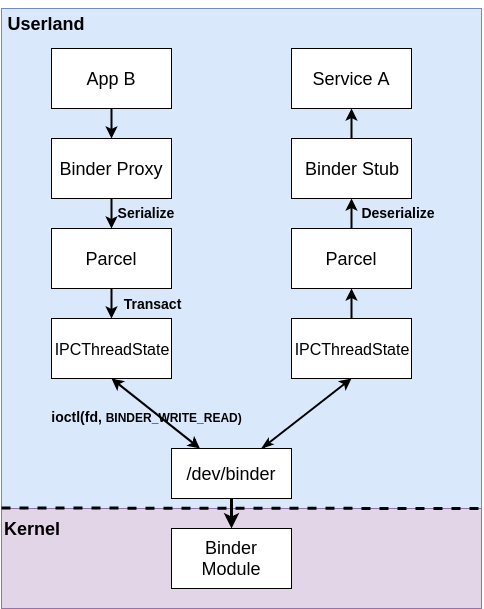
\includegraphics[width=0.49\linewidth]{\figures/binder_layers.png}
    \decoRule
    \caption[
    Layer comm]{
    Layer comm}
    \label{fig:Schéma des couches lors de la communication app/driver}
    \end{figure}




